\section{Denoise Diffusion Probabilistic Models (DDPMs)}


\subsection{Diffusion Models (DMs)}
\label{subsec:diffusion_models}

We previously talked about GANs, VAEs, and their variants (VQ-VAE, VQ-GAN). Diffusion models are also probabilistic models that define a non-linear mapping from latent variables to the observed data. Like variational autoencoders, they approximate the data likelihood using a lower bound. Diffusion models are easy to train and can produce very high-quality images compared to GANs.

A diffusion model consists of two main components: an encoder which takes a data sample $x$ and maps it through a series of intermediate latent variables $z_1, ..., z_T$, and a decoder which reverses this process, until it creates a sample image. The mappings are stochastic rather than discrete (the transformation between the latent variables involve some randomness).

In the next section, we will take a closer look at DDPMs, which is subclass of DMs. Another class of DMs is called Latent Diffusion Models (LDMs) \cite{stable_diffusion} which are based on autoencoders compressing the image space to latent space for more efficient computation.


\subsection{DDPMs}

Denoise Diffusion Probabilistic Models (DDPMs) \cite{ddpm} are a class of diffusion models that are trained to denoise images. In training phase, a dataset of images is fed to the model and DDPMs add noise to input image (it can be thought of as adding random pixel values to the input) in multiple steps (the intermediate latent variables $z_i$), unti the final result is pure noise (which will converge to the noise distribution). Then the model is trained to remove the noise and reconstruct the original image. The denoising process is called 'reverse diffusion' or reverse step and the noising process is called 'forward diffusion' or forward step. The forward diffusion step is denoted as $q(x_t | x_{t-1})$ and the reverse diffusion step is denoted as $p_\theta (x_{t-1} | x_t)$ (figure \ref{fig:ddpm_process}).

Because the addition of noise is a known stochastic process, all the learned parameters are in the decoder (the generator).

Given samples from a data distribution $q(x_0)$ we are interested in learning a model distribution $p_\theta (x_0)$ that approximates $q(x_0)$ and is easy to sample from.

DDPMs are latent variable models in the form of 

\begin{equation}
    p_\theta (x_0) = \int p_\theta(x_{0:T}) dx_{1:T} \text{,\ \ where \ \ \ } p_\theta (x_{0:T}) := p_\theta (x_T) \prod_{t=1}^{T} p_\theta (x_{t-1} | x_t)
\end{equation}

where $x_1, ..., x_T$ are latent variables. Because the integral is intractable, we use ELBO (appendix \ref{appendix:elbo}). The parameters of the model $\theta$ are learned to fit the data distribution $q(x_0)$ by maximizing a variational lower bound:

\begin{equation}
    \max_{\theta} \mathbb{E}_{q(x_0)} [\log p_\theta (x_0)] \leq \max_\theta \mathbb{E}_{q(x_0, x_1, ..., x_T)} [\log p_\theta (x_{0:T}) - \log q(x_{1:T} | x_0)]
\end{equation}

where $q(x_{1:T} | x_0)$ is some inference distribution over the latent variables. Unlike typical latent variable models (such as VAE \ref{sec:vae}), DDPMs are learned with a fixed (rather than trainable) inference procedure $q(x_{1:T} | x_0)$, and latent variables are relatively high dimensional.


\begin{figure}
    \centering
    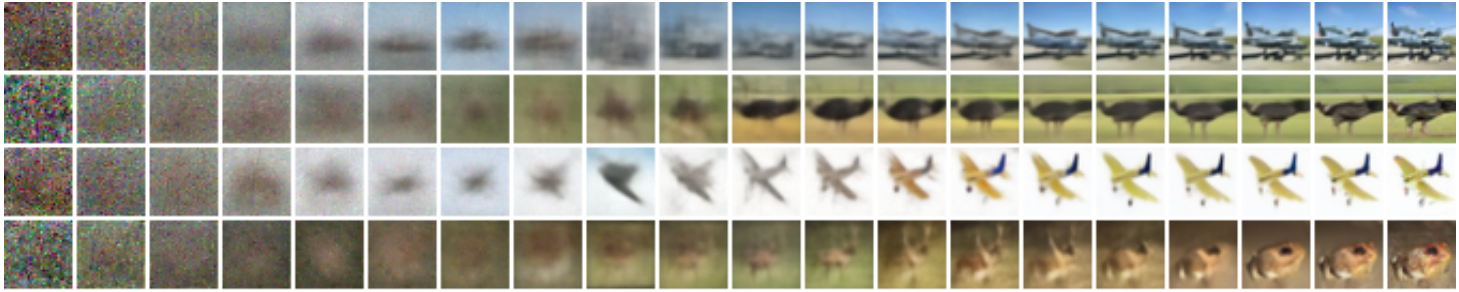
\includegraphics[width=1\textwidth]{images/diffusion_models/ddpm_denoise.png}
    \caption{Progressive generation (left to right) of unconditional CIFAR10 dataset in DDPM \cite{ddpm}.}
\end{figure}


\begin{figure}
    \centering
    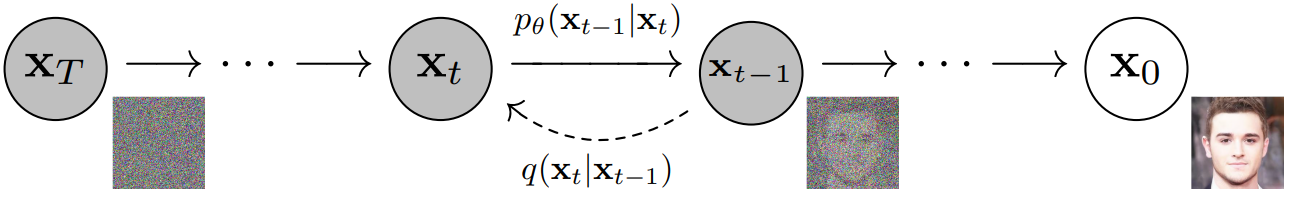
\includegraphics[width=1\textwidth]{images/diffusion_models/ddpm_process.png}
    \caption{A graph representing the forward ($q(x_t | x_{t-1})$) and reverse ($p_\theta(x_{t-1} | x_t)$) diffusion process in DDPMs \cite{ddpm}. The next step (either in forward or reverse diffusion) depends conditionally on the previous steps ($p_\theta (x_{t-1} | x_t)$ is the reverse step, and forward step is $q(x_t | x_{t-1})$).}
    \label{fig:ddpm_process}
\end{figure}






\begin{figure}[h]
    \centering
    \begin{minipage}{0.10\textwidth}  % Divide the width by 7 for 7 images
        \centering
        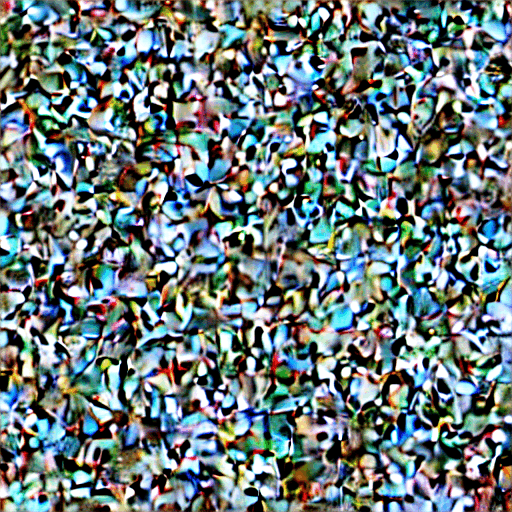
\includegraphics[width=\textwidth]{images/diffusion_models/noise_to_image_gif/0.png}
    \end{minipage}
    \begin{minipage}{0.10\textwidth}
        \centering
        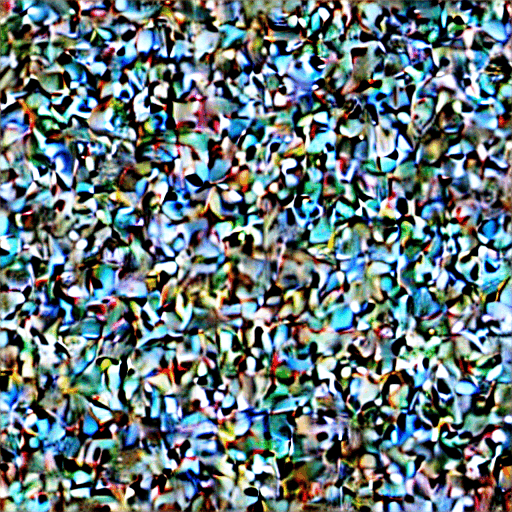
\includegraphics[width=\textwidth]{images/diffusion_models/noise_to_image_gif/1.png}
    \end{minipage}
    \begin{minipage}{0.10\textwidth}
        \centering
        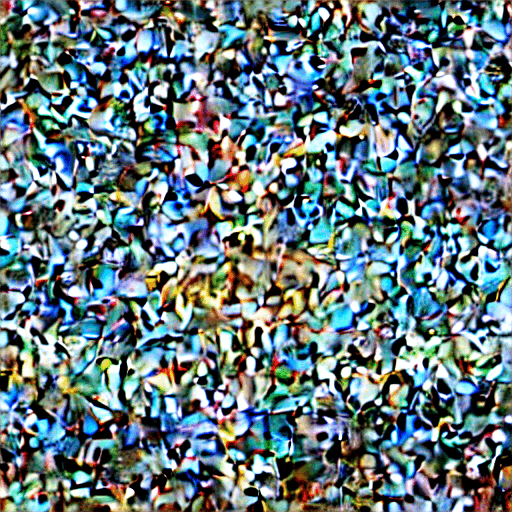
\includegraphics[width=\textwidth]{images/diffusion_models/noise_to_image_gif/2.png}
    \end{minipage}
    \begin{minipage}{0.10\textwidth}
        \centering
        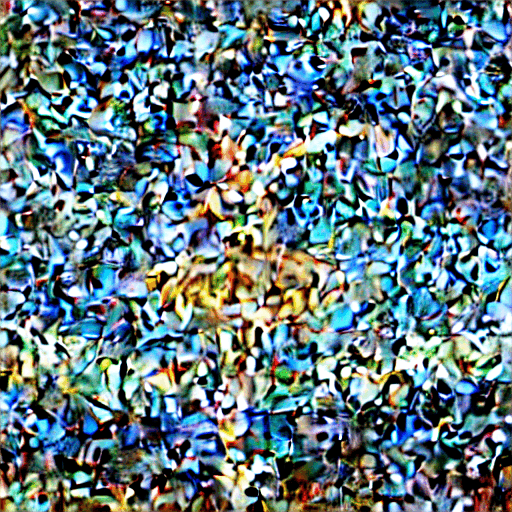
\includegraphics[width=\textwidth]{images/diffusion_models/noise_to_image_gif/3.png}
    \end{minipage}
    \begin{minipage}{0.10\textwidth}
        \centering
        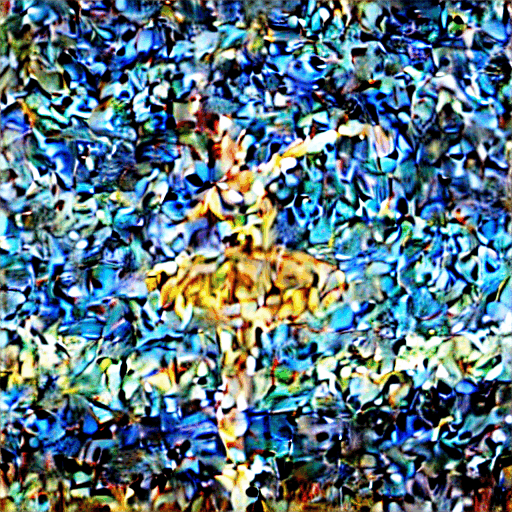
\includegraphics[width=\textwidth]{images/diffusion_models/noise_to_image_gif/4.png}
    \end{minipage}
    \begin{minipage}{0.10\textwidth}
        \centering
        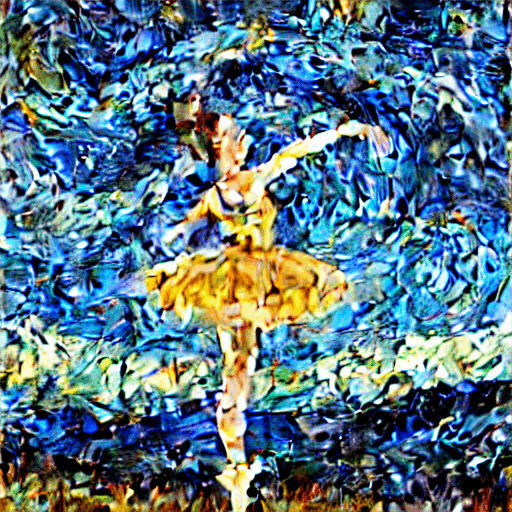
\includegraphics[width=\textwidth]{images/diffusion_models/noise_to_image_gif/5.png}
    \end{minipage}
    \begin{minipage}{0.10\textwidth}
        \centering
        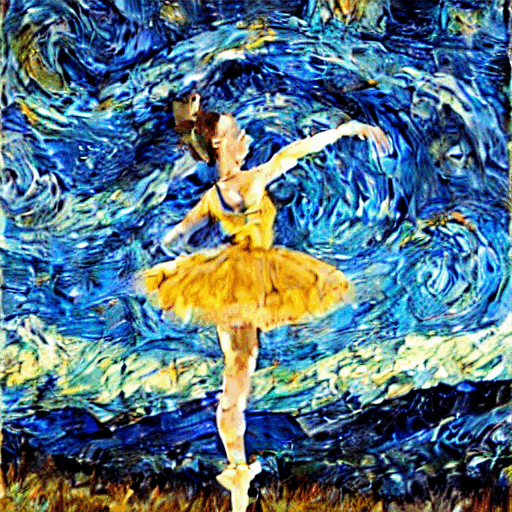
\includegraphics[width=\textwidth]{images/diffusion_models/noise_to_image_gif/6.png}
    \end{minipage}
    \begin{minipage}{0.10\textwidth}
        \centering
        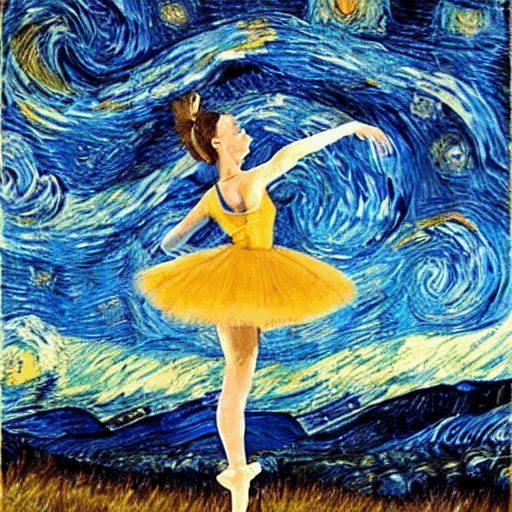
\includegraphics[width=\textwidth]{images/diffusion_models/noise_to_image_gif/7.png}
    \end{minipage}
    \caption{Progressive decoding of noise latents to an image in DDPMs \cite{ddpm}. Images taken from \href{https://scholar.harvard.edu/binxuw/classes/machine-learning-scratch/materials/stable-diffusion-scratch}{harvard university}.}
\end{figure}




\subsection{Noise Schedulers}

In the paper \cite{ddpm} the authors used linear scheduler, however OpenAI released a paper \cite{openai_improved_ddpm} that uses cosine scheduler. They have shown that a cosine scheduler performs better than a linear scheduler in terms of image generation quality (see figure \ref{fig:linear_cosine_scheduler}).

\begin{figure}
    \centering
    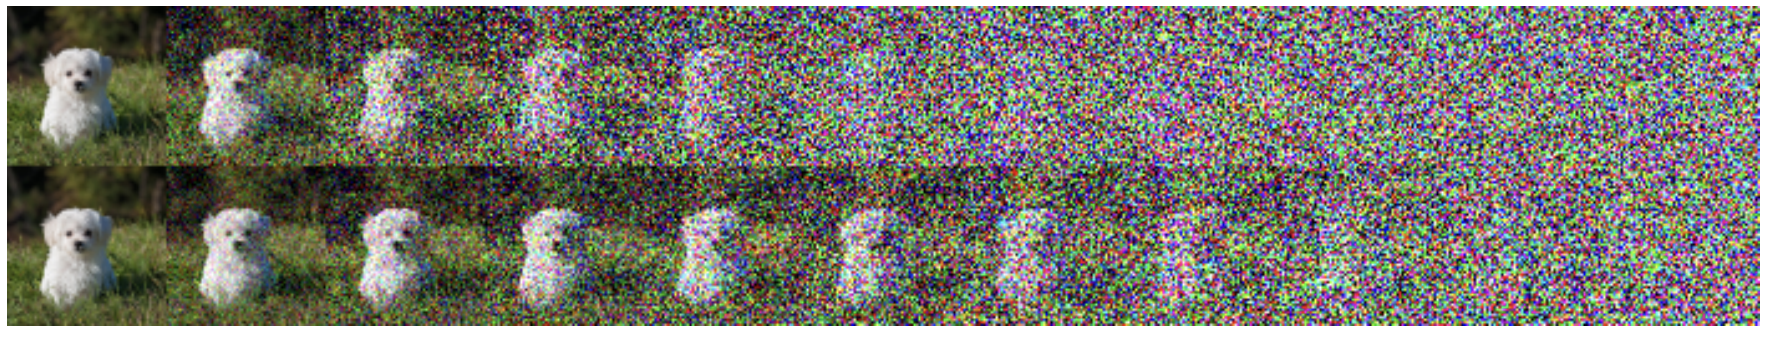
\includegraphics[width=1\textwidth]{images/diffusion_models/linear_cosine_scheduler.png}
    \caption{Linear scheduler (top, \cite{ddpm}) and cosine scheduler (bottom, \cite{openai_improved_ddpm}) shows that linear scheduler adds noise too quickly which degrades the model's performance whereas cosine scheduler adds noise more slowly.}
    \label{fig:linear_cosine_scheduler}
\end{figure}







\subsection{Encoder}

The forward diffusion process maps a data image $x$ through a series of intermediate variables $z_1, ..., z_T$ with the dimension as $x$ according to the following recursion:

\begin{equation}
    \begin{aligned}
    \mathbf{z}_1 &= \sqrt{1 - \beta_1} \cdot \mathbf{x} + \sqrt{\beta_1} \cdot \epsilon_1, \\
    &\;\;\vdots \notag \\
    \mathbf{z}_t &= \sqrt{1 - \beta_t} \cdot \mathbf{z}_{t-1} + \sqrt{\beta_t} \cdot \epsilon_t \quad \forall \, t \in \{2, \ldots, T\}
    \end{aligned}
\end{equation}

At each step $i \in {1, 2, ..., t, t+1, ..., T}$ a noise vector $e_i$ is drawn from a standard normal distribution. This equation adds random noise $e_i$ to the data (image) $x = z_0$ and $\beta$ is a schedule function ($\beta(t):[1, ..., T] \rightarrow \mathbb{R}$) that determines the amount of noise added at each step ($\beta$ is a variance schedule, which can be linear, cosine, quadratic and more). 

A more formal notation for the forward process is:

\begin{equation*}
    \begin{aligned}
        q(x_t | x_{t-1}) = \mathcal{N}(x_t; \sqrt{1-\beta_t} \cdot x_{t-1}, \beta_t \mathbf{I}) \\
        q(x_{1:T} | x_0) = \prod_{t=1}^{T} q(x_t | x_{t-1})
    \end{aligned}
\end{equation*}

In the above formula we can see that to define the next timestep $x_t$ and to get a noisier image, we define it as gaussian / normal distribution where the mean is $\sqrt{1-\beta_t} x_{t-1}$ and variance $\beta_t \mathbf{I}$. The $\beta$ parameter is the noise scheduler (how much noise we add at each step). This process is known as Markov Chain, since the next step depends only on the previous step (see appendix \ref{appendix:markov_chains}).

An interesting point the authors made is that its possible to sample $x_t$ from any arbitrary timestep $t$, given the original image $x_0$ (without calculating all the intermediate steps):

\begin{equation}
    \begin{aligned}
    q(\mathbf{x}_t|\mathbf{x}_0) = \mathcal{N}(\mathbf{x}_t; \sqrt{\bar{\alpha}_t}\mathbf{x}_0, (1 - \bar{\alpha}_t)\mathbf{I}) \\
    \text{where } \alpha_t := 1 - \beta_t \text{ and } \bar{\alpha}_t := \prod_{i=1}^{t} \alpha_i
    \end{aligned}
    \label{eq:forward_diffusion}
\end{equation}

Equation \ref{eq:forward_diffusion} describes the process of adding noise, $x_t$ from $x_0$ without any intermediate steps.

Since $\alpha$ depends on $\beta$ and $\beta$ is a noise scheduler (fixed), there are no parameters to learn in the forward process.

Each diffusion model has slightly different implementation in its network, and this encoder formulation generalizes the encoder process. We will take a closer look on the encoder/decoder network in the Stable Diffusion paper \cite{stable_diffusion} in the next section \ref{sec:stable_diffusion} and its code implementation.










\subsection{Decoder}

The decoder removes noise from the intermediate latent variables $z_1, ..., z_T$ and reconstructs the original image $x$ using the following recursion:

\begin{equation}
    p_\theta(\mathbf{x}_{t-1} | \mathbf{x}_t) = \mathcal{N}(\mathbf{x}_{t-1}; \mu_\theta(\mathbf{x}_t, t), \Sigma_\theta(\mathbf{x}_t, t))
    \label{eq:reverse_diffusion}
\end{equation}

where $\theta$ are the learned parameters of the model. The mean $\mu_\theta$ and variance $\Sigma_\theta$ are unknown and should be learned in the training stage. However, in the DDPM paper \cite{ddpm} the auhtors said:

\begin{quote}
    \textit{"We also see that learning reverse process variances (by incorporating a parameterized diagonal $\Sigma_\theta(x_t)$ into the variational bound) leads to unstable training and poorer sample quality compared to fixed variances."} \cite{ddpm}
\end{quote}

The OpenAI team released a paper titled "Improved denoising diffusion probabilistic models" \cite{openai_improved_ddpm} in which the authors used cosine noise (instead of linear in the original paper \cite{ddpm}) scheduler and also learned the variance, which significantly improved the model's performance.








\subsection{Loss function}

The loss function of DDPMs is typically the ELBO loss function (negative log-likelihood \ref{eq:elbo}):

\begin{equation*}
    \mathbb{E}[-\log p_\theta (x_0)] \leq \mathbb{E}_q[-\log \frac{p_\theta(x_{0:T})}{q(x_{1:T}|x_0)}] = \mathcal{L}
\end{equation*}

The left term is the negative log likielihood. The upper bound is the tractable ELBO loss function. The dominator $q(x_{1:T}|x_0)$ is the forward diffusion process (adds noise) and the numerator $p_\theta(x_{0:T})$ is the model's joint distribution over latent steps $x_1, ..., x_T$ which is the reverse process. The ratio of these two terms is the ELBO loss function, when this ratio reaches 1 it indicates that the model can undo the forward process. We also don't write $q_\theta$ because the forward process is not learned, only the reverse process is leanred.

Like we discussed before, diffusion models are latent variable models in the form of $p_\theta (x_0) := \int p_\theta(x_{0:T}) d\mathbf{x}_{1:T}$ which is intractable. Which is why we use the ELBO loss function to approximate the likelihood of the data (see appendix \ref{appendix:elbo}).






\subsection{Training}

The training of diffusion models is done by sampling a batch of images from the dataset, and then adding noise to the images in the forward diffusion process. The model is trained to remove the noise and reconstruct the original image in the reverse diffusion process. The loss function is the ELBO loss function (see previous section). Usually, the model is trained using stochastic gradient descent (SGD), but more advanced optimizers like Adam can be used as well.

\begin{figure}
    \centering
    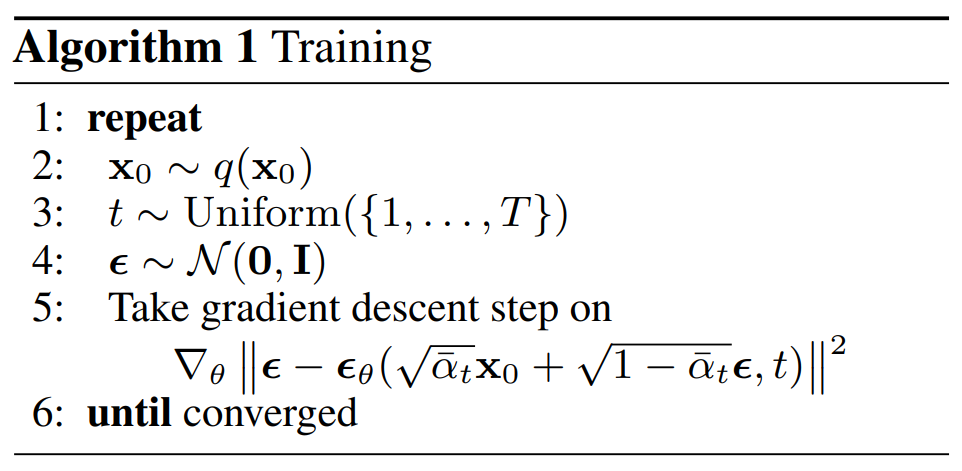
\includegraphics[width=0.5\textwidth]{images/diffusion_models/training.png}
    \caption{The training algorithm of diffusion models \cite{ddpm}. Line 2: we take a sample from the dataset. Line 3: we generate random number between 1 and T uniformly. Line 4: we sample some noise. Line 5: we calculate the gradients of the loss function.}
    \label{fig:ddpm_training}
\end{figure}

In figure \ref{fig:ddpm_training} line 5, we try to optimize the model's parameters $\theta$ by gradient decent. $\epsilon_\theta$ is the predicted noise added at timestep $t$ (a function approximator with 2 parameters that intends to predict $\epsilon$ from $x_t$) where the first parameter is the noisy image at timestep $t$, and the second parameter is the timestep ($t$). 







